%%%%%%%%%%%%%%%%%%%%%%%%%%%%%%%%%%%%%%%%%
% Beamer Presentation
% LaTeX Template
% Version 1.0 (10/11/12)
%
% This template has been downloaded from:
% http://www.LaTeXTemplates.com
%
% License:
% CC BY-NC-SA 3.0 (http://creativecommons.org/licenses/by-nc-sa/3.0/)
%
%%%%%%%%%%%%%%%%%%%%%%%%%%%%%%%%%%%%%%%%%

%----------------------------------------------------------------------------------------
%	PACKAGES AND THEMES
%----------------------------------------------------------------------------------------

\documentclass{beamer}

\mode<presentation> {
	
	% The Beamer class comes with a number of default slide themes
	% which change the colors and layouts of slides. Below this is a list
	% of all the themes, uncomment each in turn to see what they look like.
	
	%\usetheme{default}
	%\usetheme{AnnArbor}
	%\usetheme{Antibes}
	%\usetheme{Bergen}
	%\usetheme{Berkeley}
	%\usetheme{Berlin}
	%\usetheme{Boadilla}
	%\usetheme{CambridgeUS}
	%\usetheme{Copenhagen}
	%\usetheme{Darmstadt}
	%\usetheme{Dresden}
	%\usetheme{Frankfurt}
	%\usetheme{Goettingen}
	%\usetheme{Hannover}
	%\usetheme{Ilmenau}
	%\usetheme{JuanLesPins}
	%\usetheme{Luebeck}
	\usetheme{Madrid}
	%\usetheme{Malmoe}
	%\usetheme{Marburg}
	%\usetheme{Montpellier}
	%\usetheme{PaloAlto}
	%\usetheme{Pittsburgh}
	%\usetheme{Rochester}
	%\usetheme{Singapore}
	%\usetheme{Szeged}
	%\usetheme{Warsaw}
	
	% As well as themes, the Beamer class has a number of color themes
	% for any slide theme. Uncomment each of these in turn to see how it
	% changes the colors of your current slide theme.
	
	%\usecolortheme{albatross}
	%\usecolortheme{beaver}
	%\usecolortheme{beetle}
	%\usecolortheme{crane}
	%\usecolortheme{dolphin}
	%\usecolortheme{dove}
	%\usecolortheme{fly}
	%\usecolortheme{lily}
	%\usecolortheme{orchid}
	%\usecolortheme{rose}
	%\usecolortheme{seagull}
	%\usecolortheme{seahorse}
	%\usecolortheme{whale}
	%\usecolortheme{wolverine}
	
	%\setbeamertemplate{footline} % To remove the footer line in all slides uncomment this line
	%\setbeamertemplate{footline}[page number] % To replace the footer line in all slides with a simple slide count uncomment this line
	
	%\setbeamertemplate{navigation symbols}{} % To remove the navigation symbols from the bottom of all slides uncomment this line
}

\usepackage{booktabs} % Allows the use of \toprule, \midrule and \bottomrule in tables
%%%%% Packages %%%%%
\usepackage{algorithm}
\usepackage{csquotes}
\usepackage[round]{natbib}
\bibliographystyle{agsm}
\usepackage{algorithmic}
\usepackage{pgfpages}
\usepackage{ragged2e}
\usepackage{etoolbox}
\usepackage{lipsum}
\usepackage{subfig}
\apptocmd{\frame}{}{\justifying}{} 
\usepackage{xcolor}
\usepackage{dsfont}
\usepackage{tikz}
\usepackage{amsmath}
\usepackage{graphicx}
\usepackage{subfig}
\usepackage{mathtools}
\usepackage{xcolor}
\usepackage{comment}
\usepackage{appendixnumberbeamer}
%%%%% New Commands %%%%
\newcommand{\btheta}{\boldsymbol{\theta}}
\newcommand{\x}{\mathbf{x}}
\newcommand{\SUN}{\textrm{SUN}}
\newcommand{\X}{\mathbf{X}}
\newcommand{\T}{\textrm{T}}
\newcommand{\A}{\mathcal{A}}
\newcommand{\I}{\mathds{1}}
\newcommand{\hist}{\mathbb{H}_{t-1}}
\newcommand\myeq{\stackrel{\mathclap{\normalfont\mbox{def}}}{=}}
\def\app#1#2{%
	\mathrel{%
		\setbox0=\hbox{$#1\sim$}%
		\setbox2=\hbox{%
			\rlap{\hbox{$#1\propto$}}%
			\lower1.1\ht0\box0%
		}%
		\raise0.25\ht2\box2%
	}%
}
\def\approxprop{\mathpalette\app\relax}
%\pgfpagesuselayout{1 on 1}[a4paper,border shrink=5mm]

%----------------------------------------------------------------------------------------
%	TITLE PAGE
%----------------------------------------------------------------------------------------

\title[DDE and PCB effect on Premature delivery]{Assessing Effects of Exposures to DDE and PCBs on Premature Delivery via Ordinal Logistic Regression} % The short title appears at the bottom of every slide, the full title is only on the title page

\author[Morsomme, Ou, Zito]{Raphael Morsomme \and Rihui Ou \and Alessandro Zito}
\institute[Stat 723]{Case Study 1 - Stat 723}
\date{\today} % Date, can be changed to a custom date

\begin{document}
	
	\begin{frame}
	\titlepage % Print the title page as the first slide
	\end{frame}

\begin{frame}
	\frametitle{Overview} % Table of contents slide, comment this block out to remove it
	\tableofcontents % Throughout your presentation, if you choose to use \section{} and \subsection{} commands, these will automatically be printed on this slide as an overview of your presentation
\end{frame}

%----------------------------------------------------------------------------------------
%	PRESENTATION SLIDES
%----------------------------------------------------------------------------------------

%------------------------------------------------
%%%%%%%%%%%%%%%%%%%%%%%%%%%%%%%%%%%%%%%%%%%%%
%%%% Introduction                       
%%%%%%%%%%%%%%%%%%%%%%%%%%%%%%%%%%%%%%%%%%%%%
\section{Introduction}
\begin{frame}{Introduction}
\begin{itemize}
	\item \textcolor{red}{\textbf{Framework}}: \\
	\textit{Dichlorodiphenyldichloroethylene} (DDE) and \textit{Polychlorinated Biphenyls} (PCBs) 
	are chemicals that persist in the envirnoment and get stored in fatty depositis in the human tissues.\\
	$\quad \Longrightarrow \ $\textcolor{blue}{Potential adverse effect on health}
	\item \textcolor{red}{\textbf{Question}}:\\
	\textit{Is exposure to DDE and PBCs associated with a higher chance of premature delivery in pregnant women?}
\end{itemize}
\begin{block}{Pregnancy timeline}
	\begin{itemize}
		\item \textbf{Dangerous preterm}:  delivery at 34 weeks or before (when main organs are underdeveloped)
		\item \textbf{Preterm}: delivery beween 35 and 37 week
		\item \textbf{At term}: delivery after 37 weeks
	\end{itemize}
\end{block}
\end{frame}

%%%%%%%%%%%%%%%%%%%%%%%%%%%%%%%%%%%%%%%%%%%%%
%%%% The Data                       
%%%%%%%%%%%%%%%%%%%%%%%%%%%%%%%%%%%%%%%%%%%%%
\section{Data}
\begin{frame}{Data}
Data collected by 12 centers contained gestational age (in weeks) of the mother, the DDE and PCBs concentration, socio-economic info and scores (race, occupation, education, income), amount of triglycerides and cholesterol in blood and smoking status. \\
\medskip 
\textcolor{red}{\textbf{Preprocessing}}:
\begin{itemize}
	\item Drop obs. with gestational age $>$ 45 
	\item Average of standardized PCBs\footnote{This avoids the correlation between the PCBs. See the appendix.}
	$$PCB_i = \frac{1}{11}\sum_{j=1}^{11} \frac{PCB_{ij} - mean_i(PCB_{ij})}{sd_i(PCB_{ij})}$$
	\item Mean imputation of occupation, education and income scores 
	\item Aggregate race into $race = 1$ if white and $race=0$ if non-white
\end{itemize}
$\quad \Longrightarrow$ \textcolor{blue}{Total obs.} = \textbf{2336}
\end{frame}


%%%%%%%%%%%%%%%%%%%%%%%%%%%%%%%%%%%%%%%%%%%%
\begin{frame}{Data}
\small
\begin{itemize}
	\item \textbf{Ordinal dependent variable}:
	$$gestgroup_i = 
	\begin{cases}
	\textrm{Dangerous} & \text{if } \text{\#weeks} \leq 34 \\
	\textrm{Pre term } & \text{if }  34 < \text{\#weeks} \leq 37 \\
	\textrm{At term  } & \text{if }  37 < \text{\#weeks} \\
	\end{cases}$$
	\item \textbf{Adjusted measure for} $PCB$ \textbf{and} $DDE$ to estimate the level of \textit{exposure}:
	\begin{enumerate}
		\item Computing total lipids using \cite{Phillips1989} and \cite{Bernert2007} formula $$lipid_i =  2.27 * cholesterol_i + triglycerides_i + 0.623$$ 
		\item Setting\footnote{The choice of the log comes from a Box-Cox analysis of the log-likelihood, as in \cite{Li_Long_Duns}}
		$$adjDDE_i = \frac{DDE_i}{log(lipid_i)} \qquad adjPCB_i = \frac{PCB_i}{log(lipid_i)}$$
	\end{enumerate}
\end{itemize}
\end{frame}

	%%%%%%%%%%%%%%%%%%%%%%%%%%%%%%%%%%%%%%%%%%%%%
	%%%% EDA                    
	%%%%%%%%%%%%%%%%%%%%%%%%%%%%%%%%%%%%%%%%%%%%%
	\begin{frame}{EDA (I) - Exposures and gestational groups by race}
	
	\begin{figure}
		\centering
		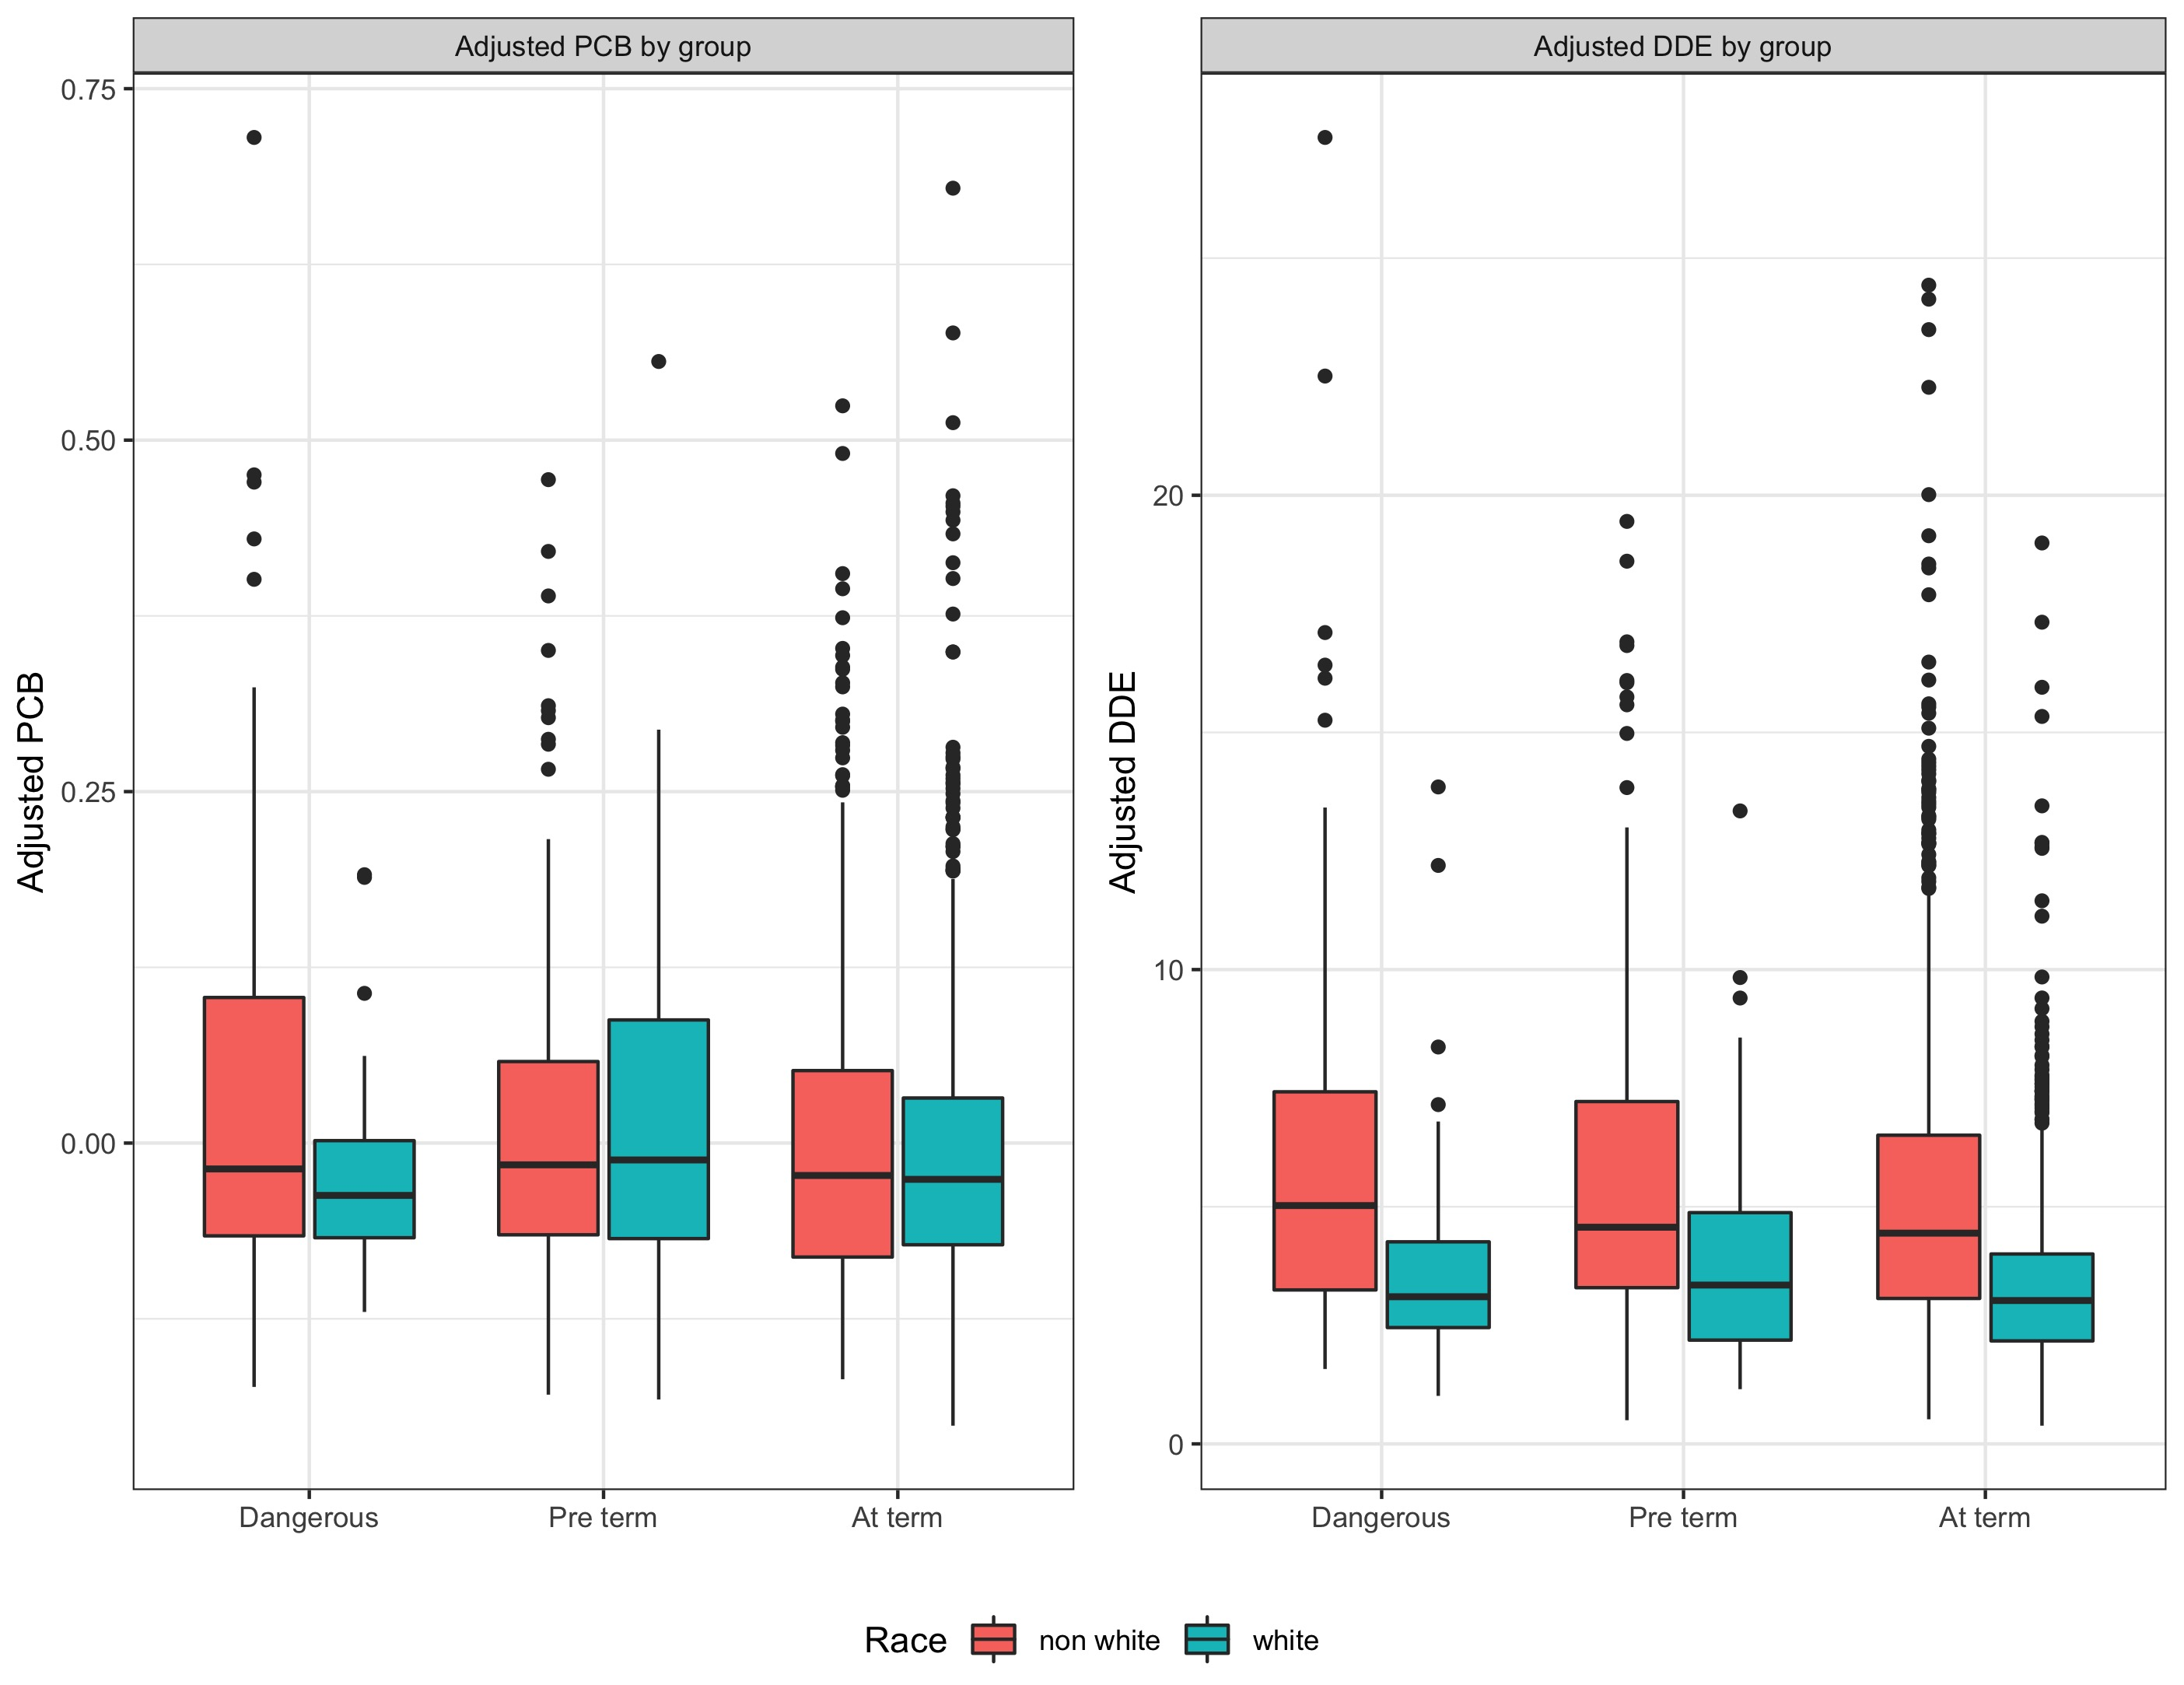
\includegraphics[width=0.8\textwidth]{pcb_dde_per_gest.jpeg}
		\caption{Relationship between gestation outcome and adjusted exposures, by race.}
		\label{fig:p1}
	\end{figure}
\end{frame}

\begin{frame}{EDA (II) - Exposure across centers}

	\begin{figure}
	\centering
	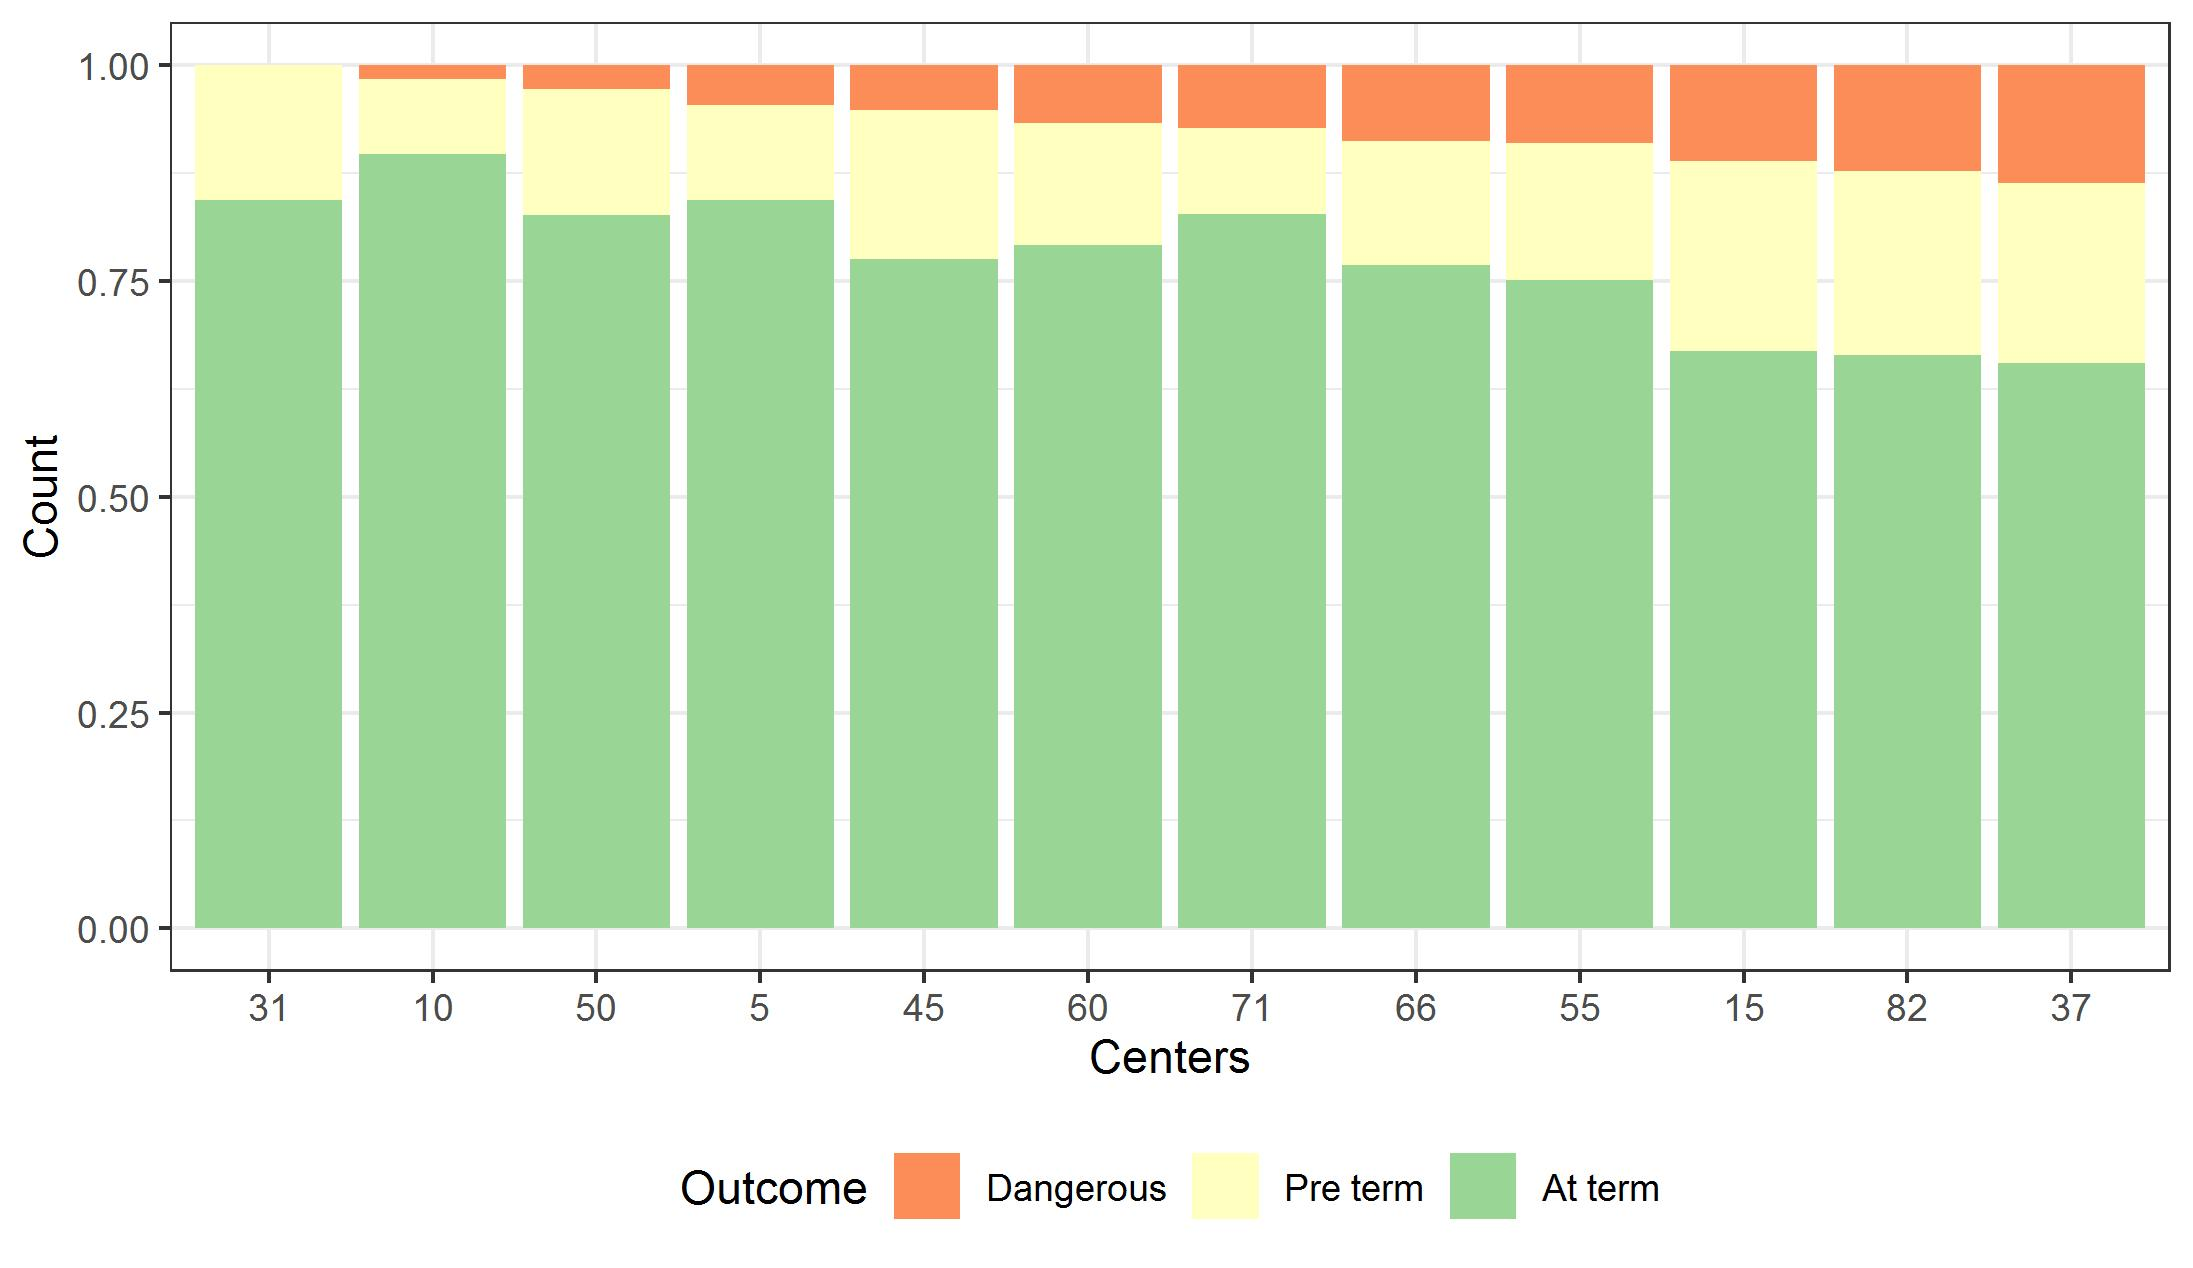
\includegraphics[width=0.8\textwidth]{outcome_per_center.jpeg}
	\caption{Distribution of gestation outcome per center.}
	\label{fig:p1}
\end{figure}

\end{frame}



%%%%%%%%%%%%%%%%%%%%%%%%%%%%%%%%%%%%%%%%%%%%%
%%%% Model 1                    
%%%%%%%%%%%%%%%%%%%%%%%%%%%%%%%%%%%%%%%%%%%%%
\section{Model (I) - Ordinal Logistic Regression}

% Insert here the AIC part
\begin{frame}{Model - Ordinal Logistic Regression}
We run the following ordinal logistic regression model:
\begin{align*}
\textrm{logit}(P(gestgroup \leq j)) = \beta_{0j} - \mathbf{X} \boldsymbol{\beta}
\end{align*}

where $j = 0,1$ corresponds to the outcome level, and \textbf{X} contains:
\begin{itemize}
	\item $DDE$, $PCB$, $race$, $center$, $smoke$, the 3 scores, mother age [\textcolor{blue}{main effects}]
	\item ($adjDDE$ + $adjPCB$) * ($race$ + $center$) [\textcolor{blue}{interactions}].
\end{itemize}

\end{frame}


\begin{frame}{Model - Inference}

Bayesian ordinal logistic regression using the variables selected by AIC-based backward variable selection procedure.
\begin{itemize}
	\item \textcolor{blue}{Maintain} $DDE$, $PCB$, $smoke$, $center$, $race$, ($PCB$ + $DDE$) * $race$
	\item \textcolor{red}{Drop} 3 scores, ($DDE$ + $PCB$) * $center$ , mother age
	\item uniform, and $R^2$ prior on coefficients
	\item Model assumptions are checked in the appendix.
\end{itemize}


\end{frame}



% https://www.ncbi.nlm.nih.gov/pmc/articles/PMC3812826/#R13

%%%%%%%%%%%%%%%%%%%%%%%%%%%%%%%%%%%%%%%%%%%%%
%%%% Results
%%%%%%%%%%%%%%%%%%%%%%%%%%%%%%%%%%%%%%%%%%%%%
\section{Results}

\begin{frame}{Numerical Results}
\begin{table}
\centering
\begin{tabular}{l|r|r|r}
\hline
  & mean & 5\% & 95\%\\
\hline
adjDDE & 0.02 & -0.01 & 0.05\\
\hline
adjPCB & 1.76 & 0.72 & 2.75\\
\hline
adjDDE*white & 0.05 & -0.02 & 0.12\\
\hline
adjPCB*white & -1.60 & -3.26 & 0.02\\
\hline
\end{tabular}
\end{table}
\medskip
\small
\textcolor{red}{\textbf{Interpretation:}}\\
For a 1 unit increase of \textcolor{blue}{adjDDE}: 
\begin{itemize}
\item \textbf{Nonwhite}: the odds of having a more dangerous delivery increase by $(e^{(0.02)}-1)*100\%=2.02\%$ 
\item \textbf{White}:  the same odds increase by $(e^{(0.02+0.05)}-1)*100\%=7.25\%$
\end{itemize}
For a $0.1$ unit increase of \textcolor{blue}{adjPCB}:
\begin{itemize}
\item \textbf{Nonwhite}: the odds of having a more dangerous delivery increase by $(e^{(1.76)*0.1}-1)*100\%=19.22\%$
\item \textbf{White}:  the same odds increase by $(e^{0.1*(1.76-1.60)}-1)*100\%=1.595\%$
\end{itemize}

\end{frame}
%%%%%%%%%%%%%%%%%%%%%%%%%%%%%%%%%%%%%%%%%%%%%
%%%% Results
%%%%%%%%%%%%%%%%%%%%%%%%%%%%%%%%%%%%%%%%%%%%%
\section{Results}

\begin{frame}{Graphical Results}
\begin{figure}
	\centering
	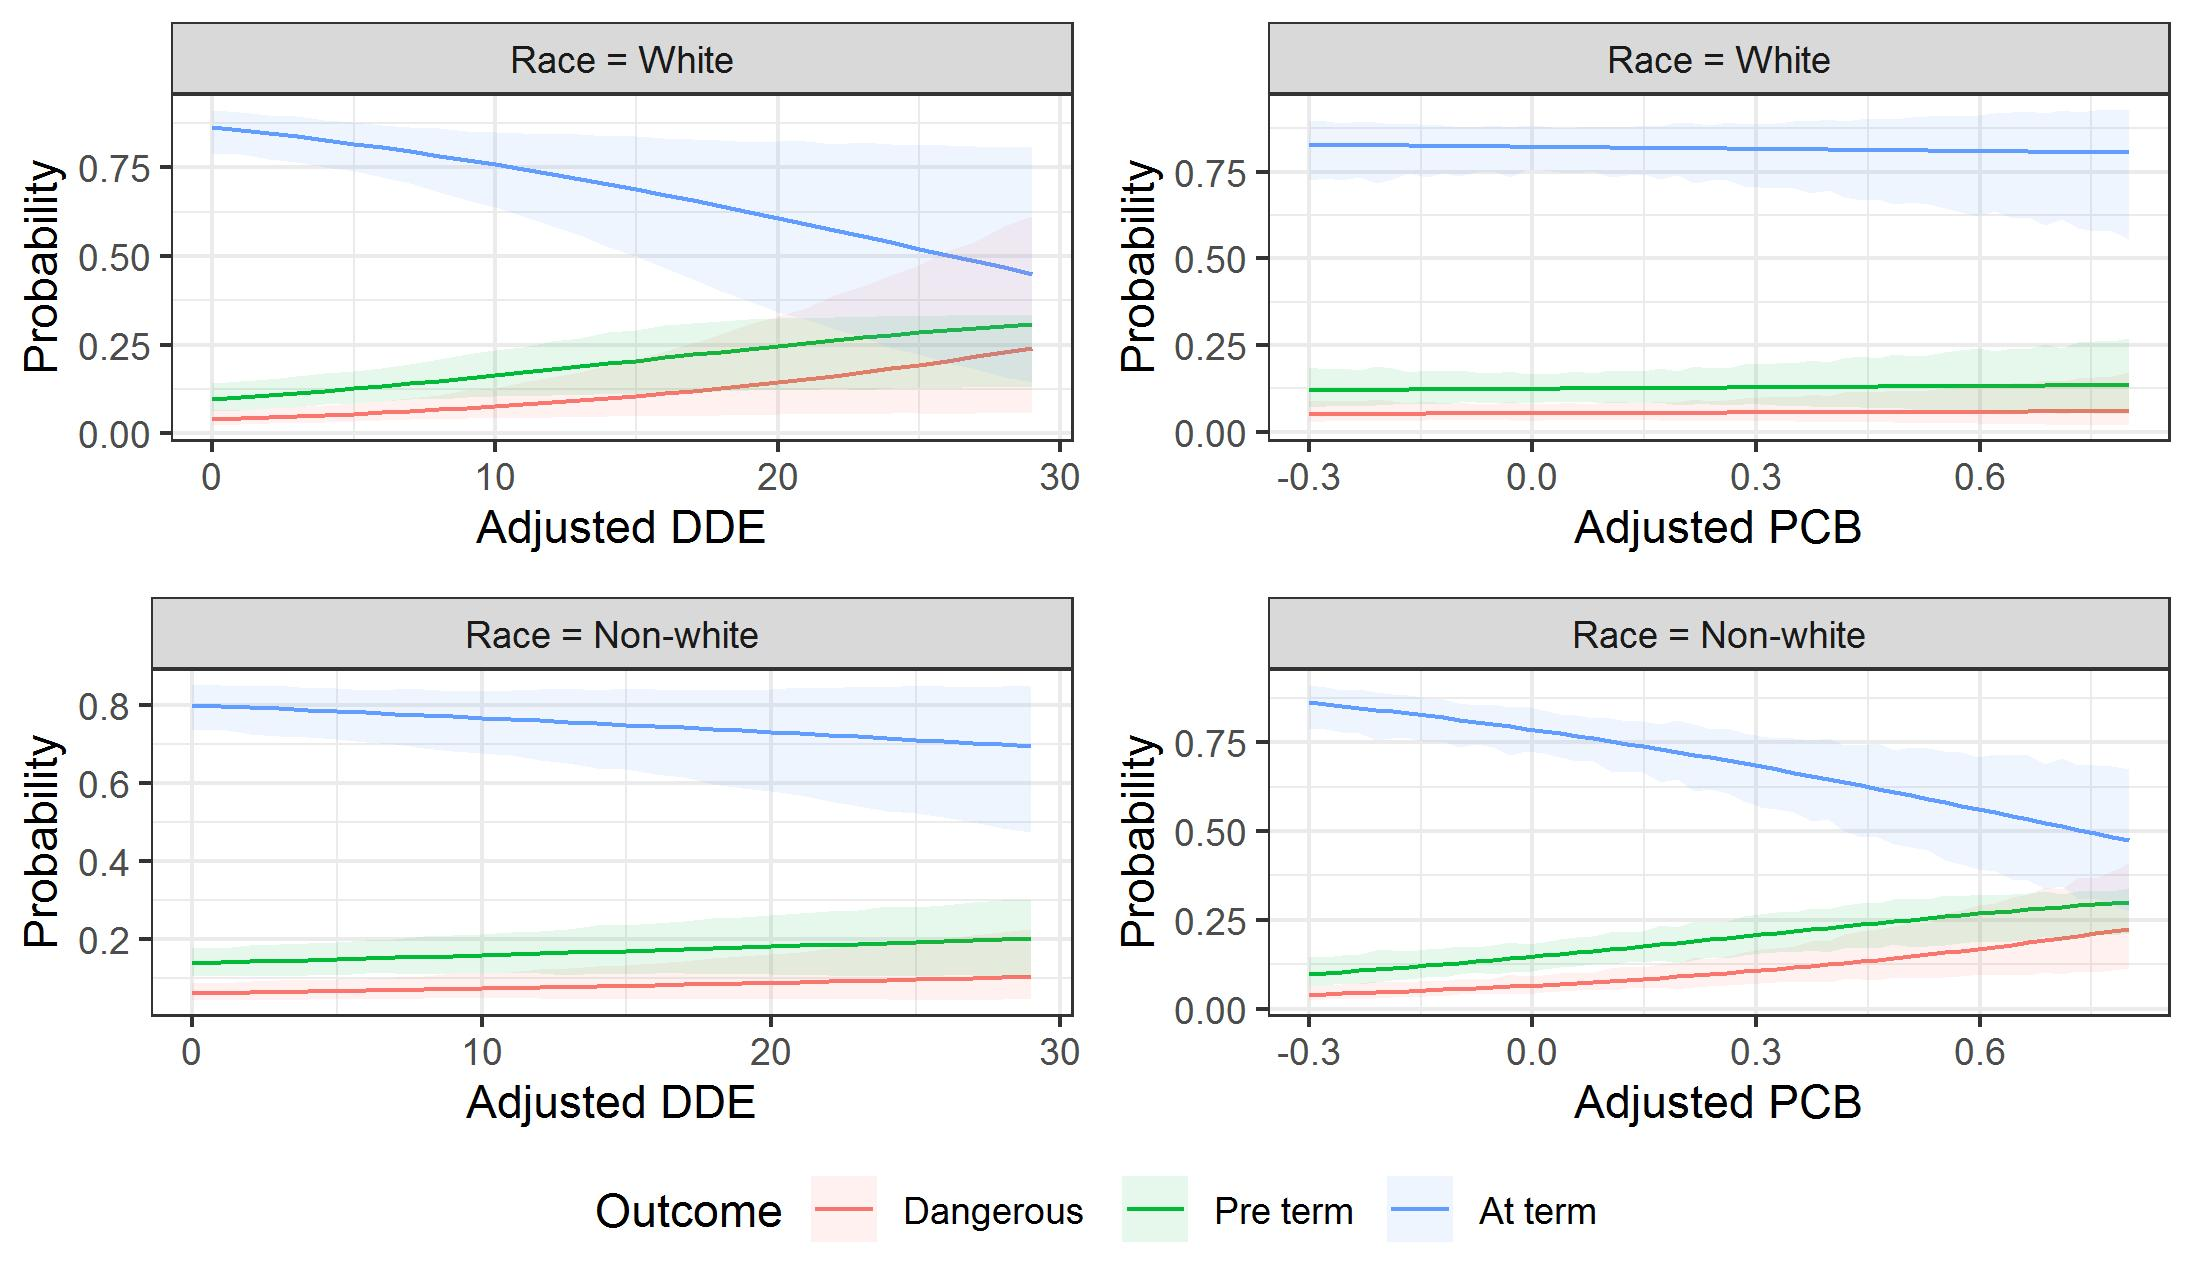
\includegraphics[width=1\textwidth]{results.jpeg}
	\caption{Estimated probability of gestation outcomes for DDE and PCB, by race.}
	\label{fig:corrPCB}☺
\end{figure}

\end{frame}

%%%%%%%%%%%%%%%%%%%%%%%%%%%%%%%%%%%%%%%%%%%%%
%%%% Conclusions                  
%%%%%%%%%%%%%%%%%%%%%%%%%%%%%%%%%%%%%%%%%%%%%

\section{Conclusions}
\begin{frame}{Conclusions}
To summarize:
\begin{itemize}
	\item Effect of the chemicals is race-dependent
	\item DDE has more impact on white people
	\item PCB has more impact on non-white people
\end{itemize}
\end{frame}


\begin{frame}
\frametitle{References}
\footnotesize{
	\begin{thebibliography}{99} % Beamer does not support BibTeX so references must be inserted manually as below
		
		\bibitem[Li et al, 2013]{Li_Long_Duns} Li, D; Longnecker, M.P.; and Dunson, D.B. \\
		\newblock Lipid Adjustment for Chemical Exposures: Accounting for Concomitant Variables.\\
		\newblock \emph{Epidemiology}, Nov 2013
		
		\bibitem[Phillips et al.(1989)]{Phillips1989}Phillips, D; Pirke, J., Burse, V.; Bernert, J.; Henderson, L.; Needham, L.\\
		\newblock Chlorinated hydrocarbon levels in human serum: Effects of fasting and feeding.\\
		\newblock \emph{Archives of Environmental Contamination and Toxicology}, 1989
		
		\bibitem[Bernert et al, 2007]{Bernert2007} Bernert, JT.; Turner, WE.;, Patterson, DG. Jr;, Needham, LL.\\
		\newblock Calculation of serum total lipid concentrations for the adjustment of persistent organohalogen toxicant measurements in human samples.\\
		\newblock \emph{Chemosphere}, 2007
		
		\bibitem[Liu and Zhang, 2018]{Liu2018} Liu, D.; and Zhang, H.;\\
		\newblock Residuals and Diagnostics for Ordinal Regression Models: A Surrogate Approach\\
		\newblock \emph{Journal of the Americal Statistical Association}, 2018
		
	\end{thebibliography}
}
\end{frame}
%%%%%%%%%%%%%%%%%%%%%%%%%%%%%%%%%%%%%%%%%%%%%
%%%% Appendix                 
%%%%%%%%%%%%%%%%%%%%%%%%%%%%%%%%%%%%%%%%%%%%%
\appendix
\section{Appendix}
\begin{frame}{Appendix}{More EDA}
\begin{figure}
\centering
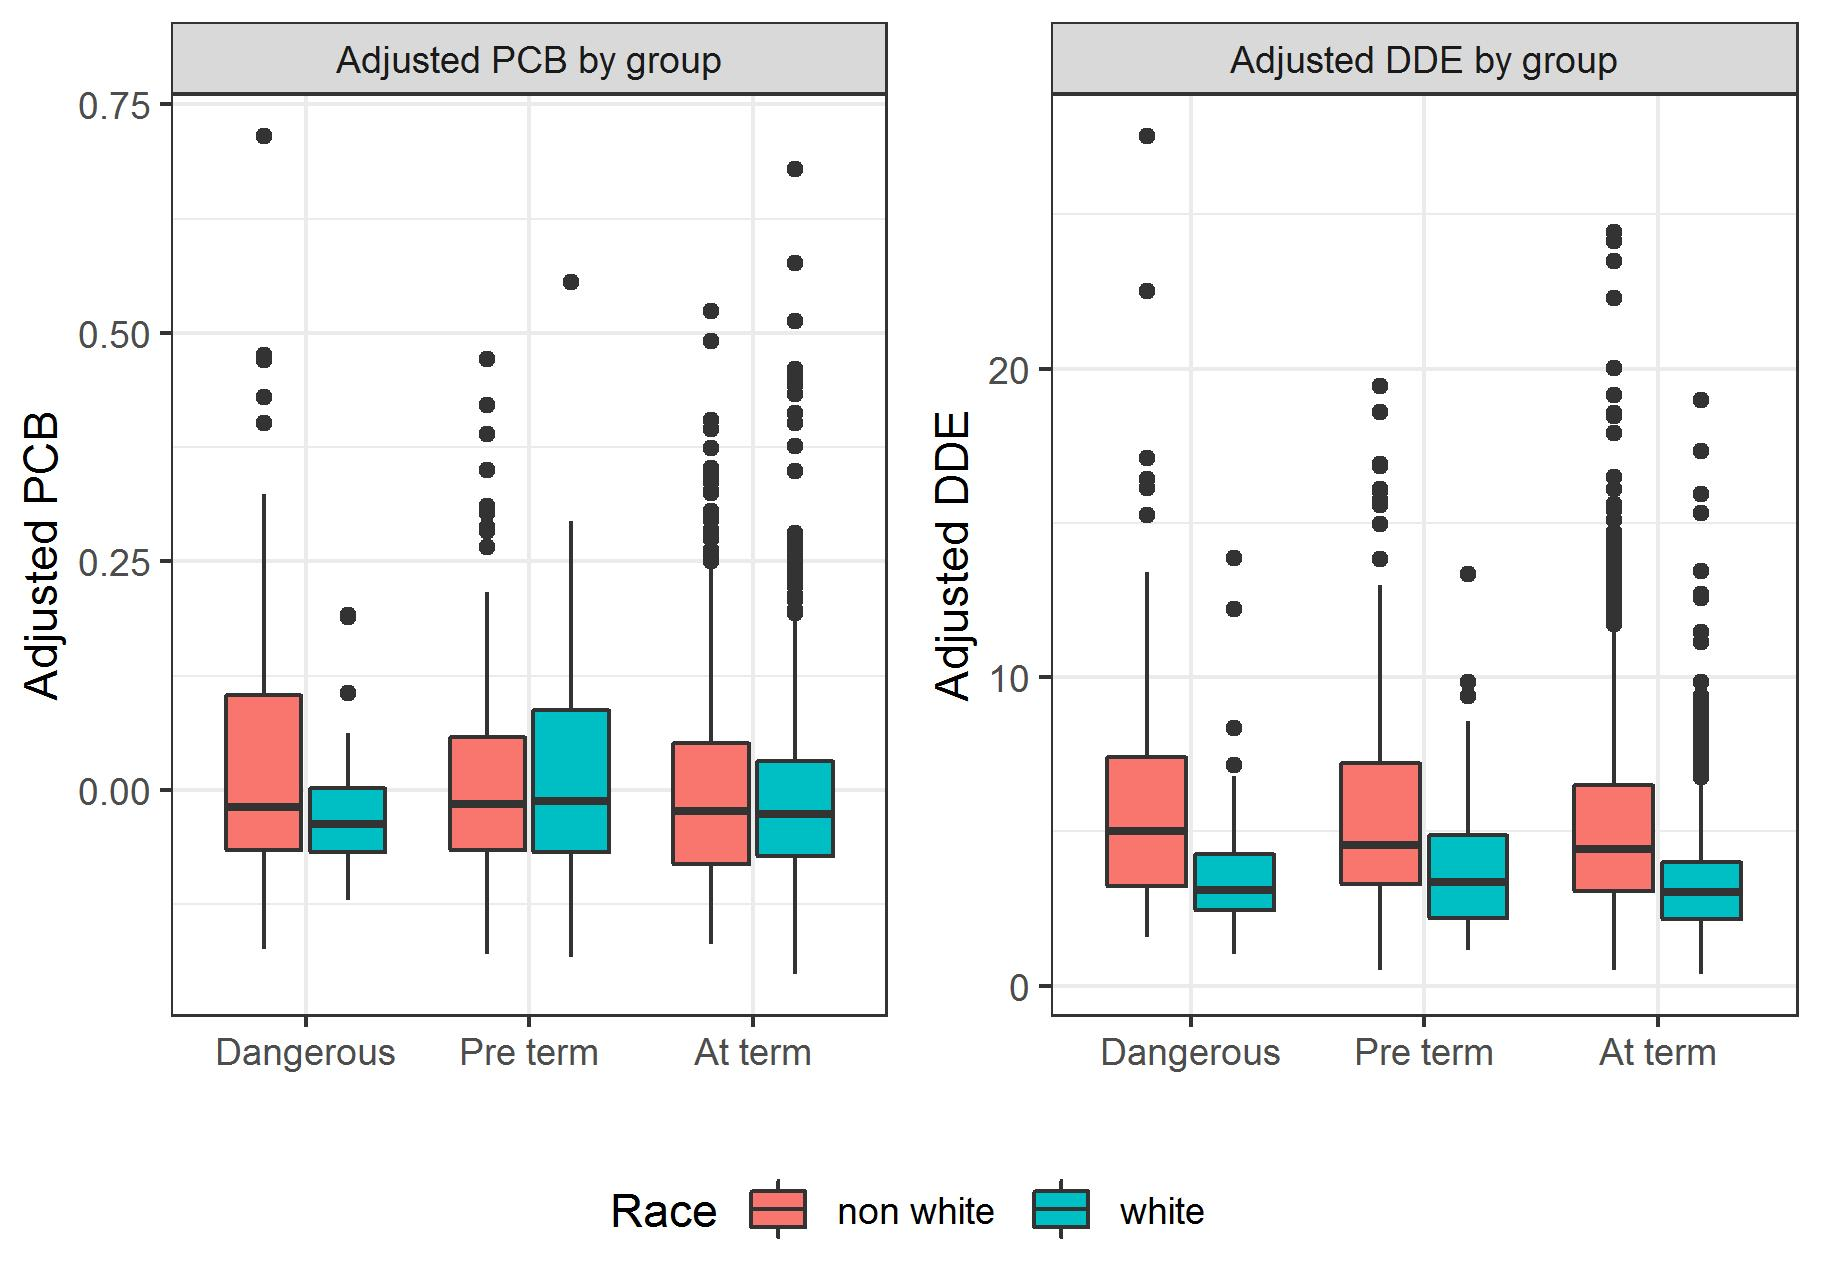
\includegraphics[width=0.6\textwidth]{pcb_corr.jpeg}
\caption{Correlation plot across PCBs}
\label{fig:corrPCB}
\end{figure}
\end{frame}
%%%%%%%%%%%%%%%%%%%%%%%%%%%%%%%%%%%%%%%%%%%%%
\begin{frame}{Appendix}{Frequentist Model Checking}

We can check the assumption of the (frequentist) ordinal logistic model by looking at the Surrogate residuals (Liu and Zhang, 2018).\\

\medskip
If the model assumptions are correct, then the surrogate residuals $R_S$ will have three properties:
\begin{enumerate}
\item $E(R_S|X)=0$
\item $Var(R_S|X)=c$, the conditional variance of $R_S$ is constant
\item The emiprical distribution of $R_S$ resembles an explicit distribution that is related to the link function $G^{-1}(\cdot)$. Specifically, $R_S\sim G(c+\int ud G(u))$.
\end{enumerate}
\end{frame}
%%%%%%%%%%%%%%%%%%%%%%%%%%%%%%%%%%%%%%%%%%%%%
\begin{frame}{Appendix}{Frequentist Model Checking}
Assumptions (i) and (ii) are checked with the Surrogate residuals plot. Both are satisfied in this case.
\begin{figure}
\centering
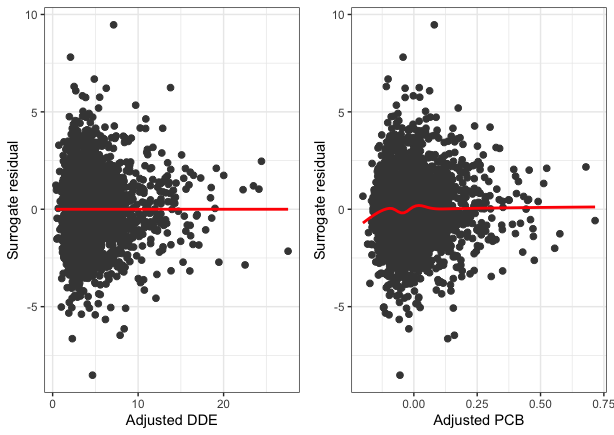
\includegraphics[width=0.7\textwidth]{Surrogate_residuals.png}
\caption{Surrogate residuals of DDE and PCB}
\label{fig:surrogateresid}
\end{figure}
\end{frame}
%%%%%%%%%%%%%%%%%%%%%%%%%%%%%%%%%%%%%%%%%%%%%
\begin{frame}{Appendix}{Frequentist Model Checking}
\begin{figure}
\centering
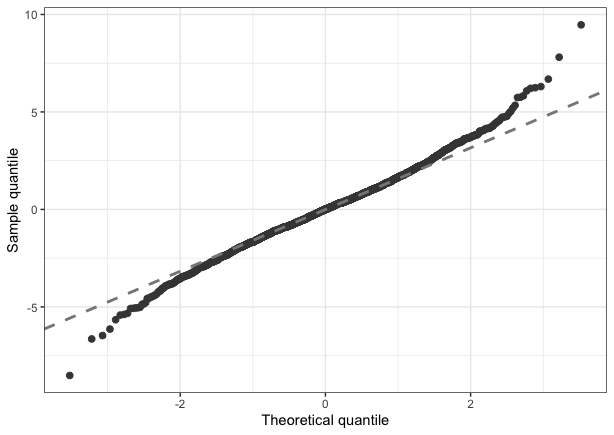
\includegraphics[width=0.7\textwidth]{qqplot.png}
\caption{QQ plot of the Surrogate residuals}
\label{fig:qqplot}
\end{figure}
\end{frame}

\end{document} 